\chapter{音声合成}
\section{\kadaica}\label{sec:\kadaica}
\purpose
ノコギリ波は,矩形波と同様周期関数である.ゆえにノコギリ波は\eqref{equ:フーリエ級数展開}で表すことができる.矩形波とノコギリ波は合成波である.\par
この実験ではノコギリ波と矩形波の,初期位相の変化に対して波形の変化と音の変化を確かめる.初期位相の変化は,固定値と高調波成分ごとにランダムな値で確かめる.

\begin{wrapfigure}{r}[0mm]{.3\textwidth}
    \centering
    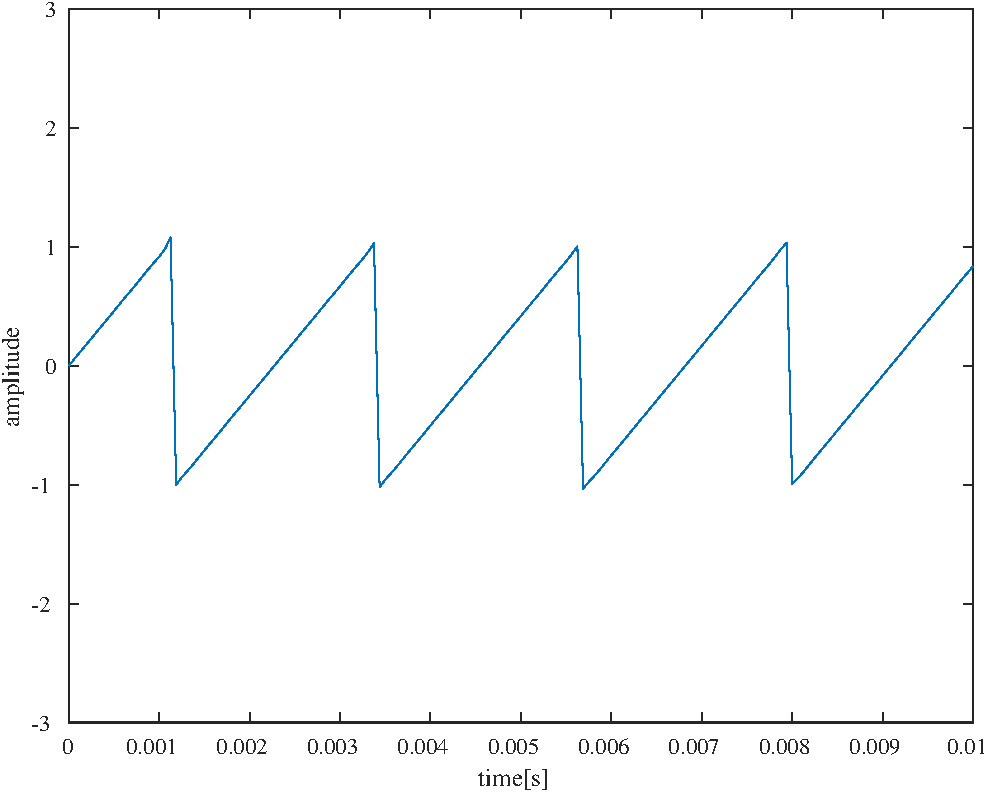
\includegraphics[keepaspectratio,width=.3\textwidth]{../../Figures/03_11_nokogiri.pdf}
    \caption{ノコギリ波\ \((N=50)\)}
    \label{fig:ノコギリ波}
    \begin{lstlisting}[caption={ランダム初期位相},label={src:ランダム初期位相},numbers={none}]
for k=1:50
 y =y+sin(2*pi*f*t+rand);
end    
    \end{lstlisting}
    \vspace{-2cm}
\end{wrapfigure}
\method
\paragraph{ノコギリ波}ノコギリ波は\eqref{equ:noko1}を周期\(2\pi\)の関数として周期的に\eqref{equ:noko2}へ拡張したものであり,ノコギリ波をフーリエ級数展開すると,\eqref{equ:ノコギリ波}の\(N=\infty\)で表せる.
\begin{align}
    f(t) & =t\label{equ:noko1}                                                                               \\
    f(t) & =f(t+2k\pi)                                                   & (k\in\mathbb{Z})\label{equ:noko2} \\
    f(t) & =\sum_{k=1}^{N}(-1)^{k-1}\frac{2}{k}\sin(kt)\label{equ:ノコギリ波}
\end{align}
\paragraph{乱数の生成}乱数の生成は\matlab の\texttt{rand}関数を用いる.\texttt{rand}関数は引数や演算を与えない状態(\texttt{r = rand})で用いると,区間\((0,1)\)の一様分布から取り出された乱数スカラを返す\cite{matlab_rand}.
今回は,引数や演算を与えずに\texttt{rand}関数を用いる.\par
波形に高調波成分ごとのランダムな初期位相を与えるためには,繰り返し処理の都度\texttt{rand}関数を呼び出すと良い(\srcref{src:ランダム初期位相}).
\paragraph{実験の内容}今回の実験では,ノコギリや初期位相に対して,固定値の初期位相\(\pi/4\),\(\pi/2\)を与え,高調波ごとにランダムな初期位相を与える.また,\eqref{equ:矩形波},\eqref{equ:ノコギリ波}ともに\(N=50\)として実装する.
\scall\sref{src:03_01_1},\sref{src:03_01_2}.
\result
\paragraph{矩形波}
音の波形を\figref{fig:矩形波の初期位相}に示す.聴音確認の結果,\figref{fig:実験結果矩形波_pure}に比べて,\figref{fig:実験結果矩形波_p2PI},\figref{fig:実験結果矩形波_p4PI}の方が滑らかな音に聞こえた.
\figref{fig:実験結果矩形波_pure}と\figref{fig:実験結果矩形波_rand}の音は似ていた.矩形波は純音に比べて,掠れた音が聞こえた.音量について,\figref{fig:実験結果矩形波_p2PI},\figref{fig:実験結果矩形波_p4PI}は\figref{fig:実験結果矩形波_pure}の\(3/4\)程度の音量に聞こえた.\figref{fig:実験結果矩形波_pure}と\figref{fig:実験結果矩形波_rand}の音量変化は確認できなかった.
\paragraph{ノコギリ波}
音の波形を\figref{fig:ノコギリ波の初期位相}に示す.聴音確認の結果,\figref{fig:実験結果ノコギリ波_pure}に比べて,矩形波と同様に\figref{fig:実験結果ノコギリ波_p2PI},\figref{fig:実験結果ノコギリ波_p4PI}の方が滑らかな音に聞こえた.
\figref{fig:実験結果ノコギリ波_pure}と\figref{fig:実験結果ノコギリ波_rand}の音は似ていた.ノコギリ波は純音に比べて,尖った音が聞こえた.音量について,\figref{fig:実験結果矩形波_p2PI},\figref{fig:実験結果ノコギリ波_p4PI}は\figref{fig:実験結果ノコギリ波_pure}の\(3/4\)程度の音量に聞こえた.\figref{fig:実験結果ノコギリ波_pure}と\figref{fig:実験結果ノコギリ波_rand}の音量変化は確認できなかった.
\paragraph{波形}初期位相を固定値で与えると,初期位相が\(0\)の波形とは異なる波形を示す.
\begin{figure}[H]
    \centering
    \begin{minipage}[b]{.24\textwidth}
        \centering
        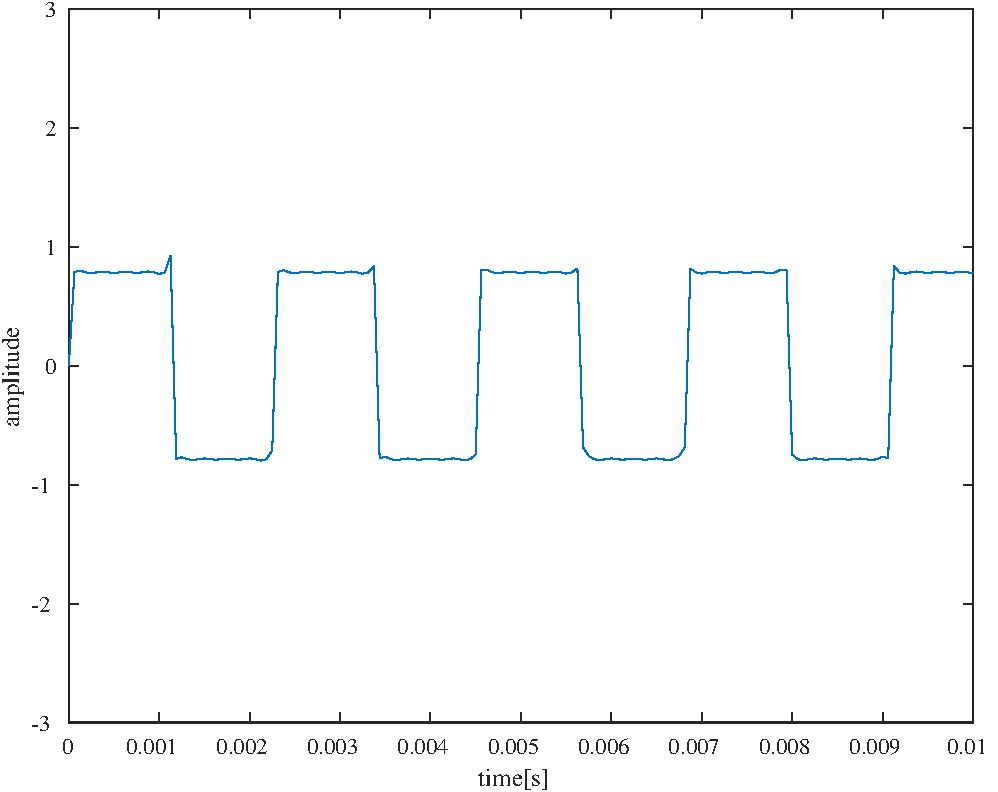
\includegraphics[keepaspectratio,width=\textwidth]{../../Figures/03_11_kukei.pdf}
        \subcaption{矩形波}
        \label{fig:実験結果矩形波_pure}
    \end{minipage}
    \begin{minipage}[b]{.24\textwidth}
        \centering
        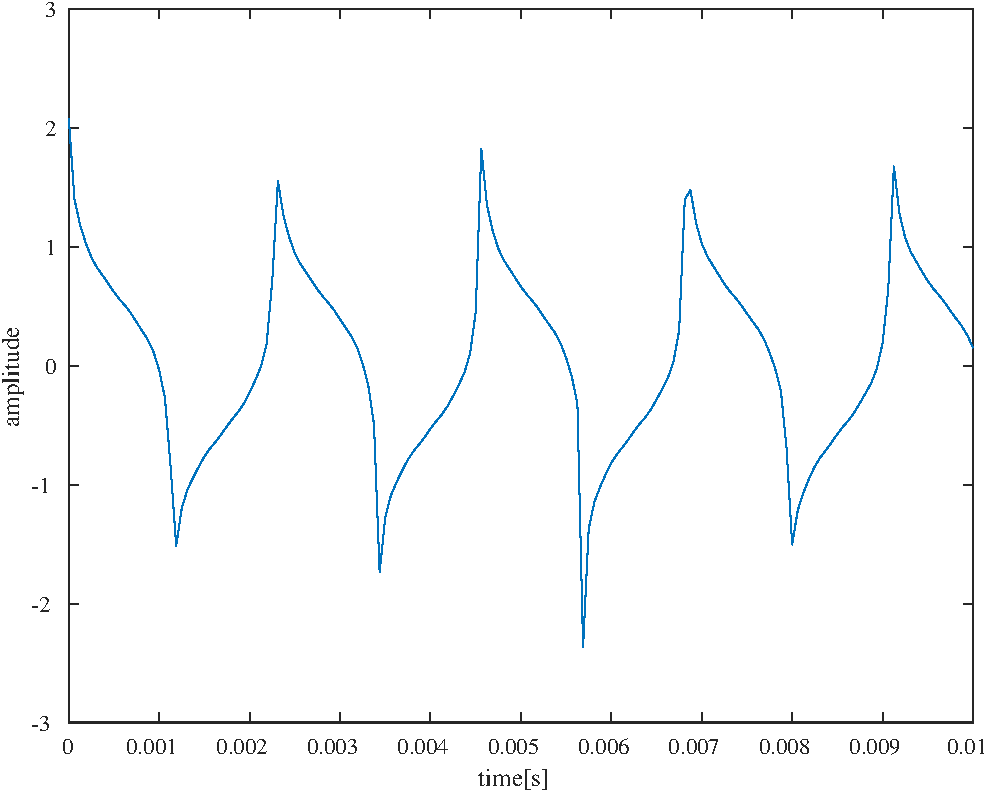
\includegraphics[keepaspectratio,width=\textwidth]{../../Figures/03_12.pdf}
        \subcaption{初期位相\ \(+\pi/4\)}
        \label{fig:実験結果矩形波_p4PI}
    \end{minipage}
    \begin{minipage}[b]{.24\textwidth}
        \centering
        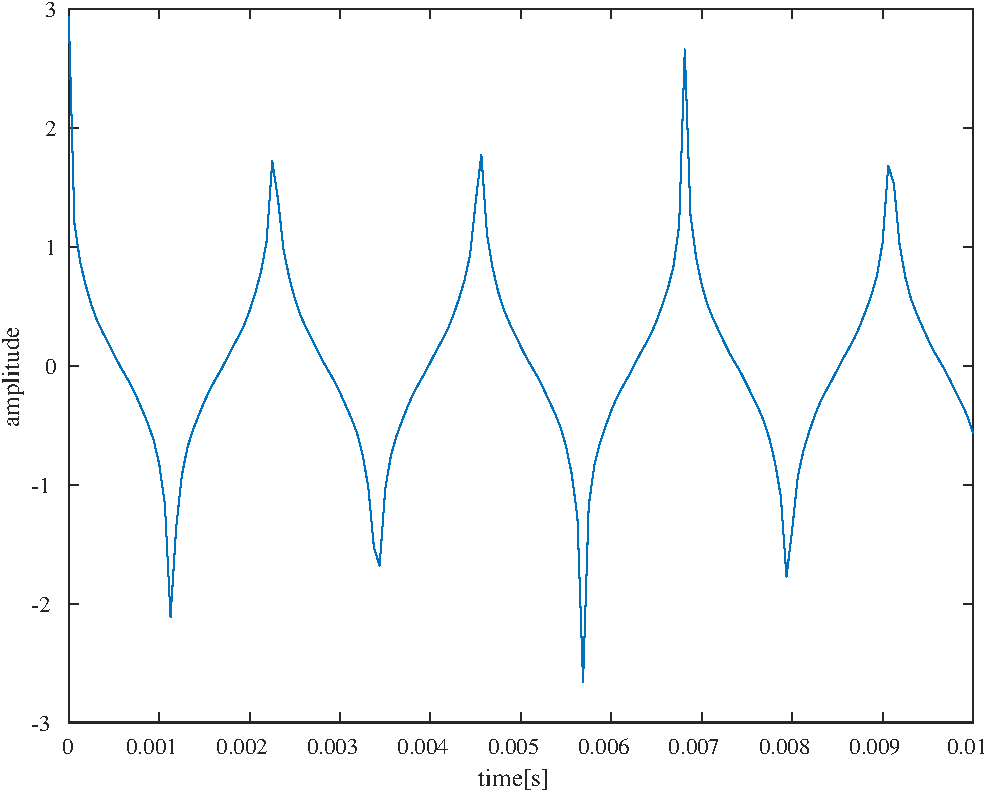
\includegraphics[keepaspectratio,width=\textwidth]{../../Figures/03_13.pdf}
        \subcaption{初期位相\ \(+\pi/2\)}
        \label{fig:実験結果矩形波_p2PI}
    \end{minipage}
    \begin{minipage}[b]{.24\textwidth}
        \centering
        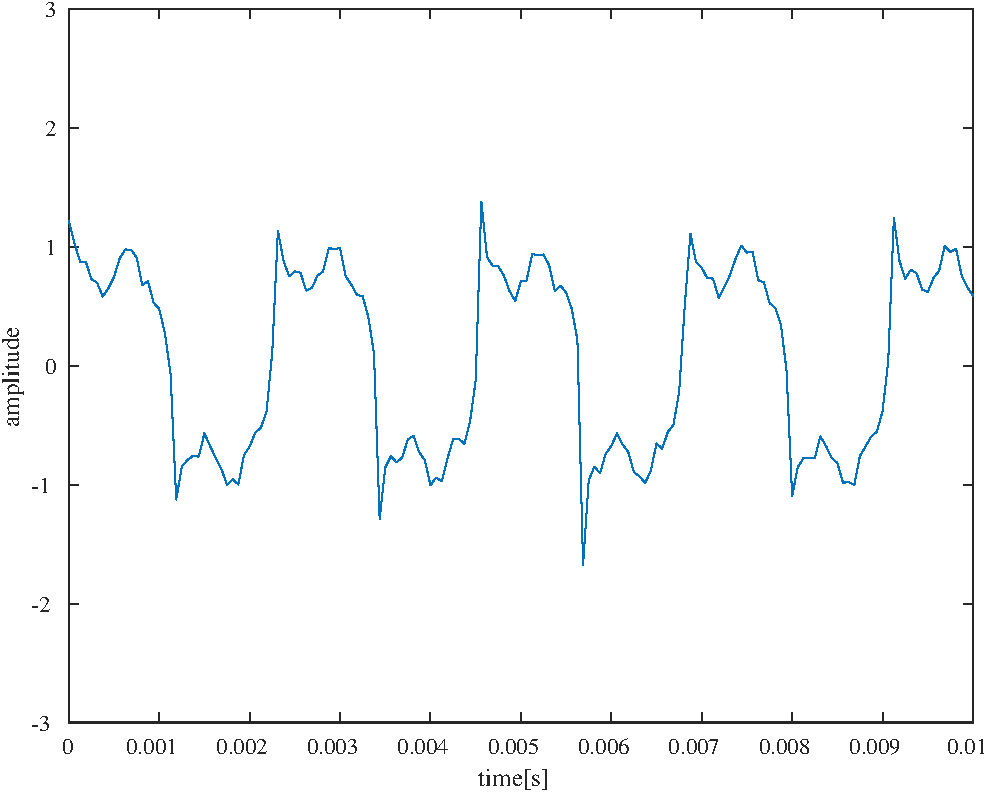
\includegraphics[keepaspectratio,width=\textwidth]{../../Figures/03_14.pdf}
        \subcaption{初期位相\ \texttt{rand}}
        \label{fig:実験結果矩形波_rand}
    \end{minipage}
    \caption{矩形波の初期位相}
    \label{fig:矩形波の初期位相}
    \begin{minipage}{.24\textwidth}
        \centering
        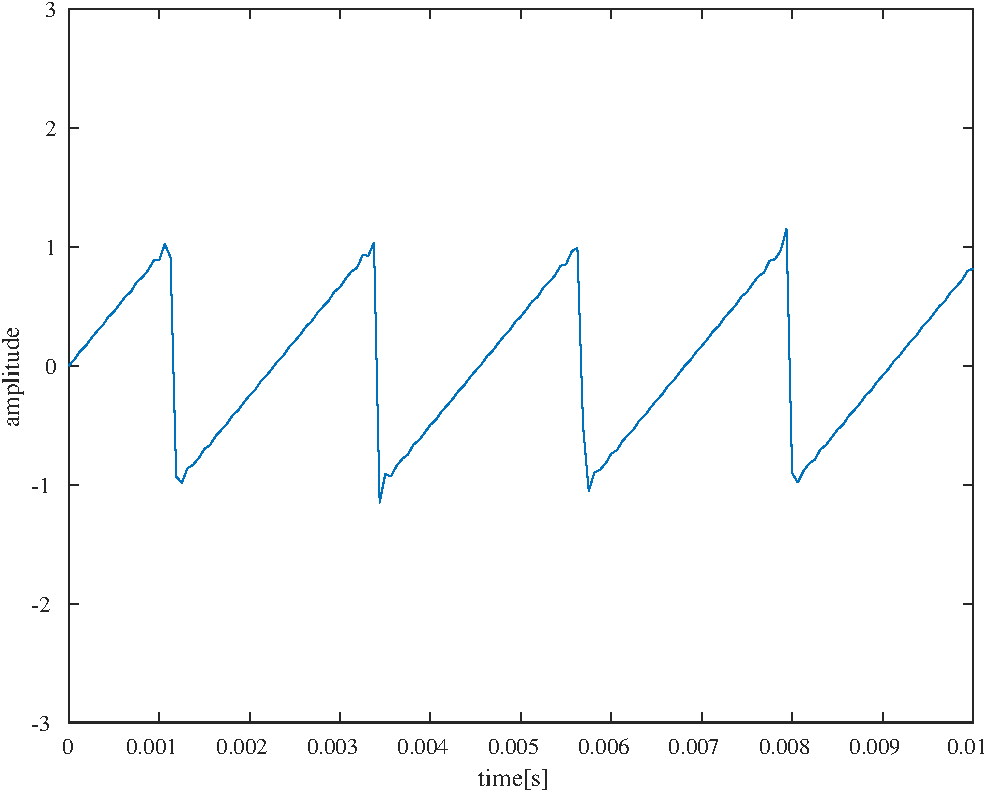
\includegraphics[keepaspectratio,width=\textwidth]{../../Figures/03_21_nokogiri.pdf}
        \subcaption{ノコギリ波}
        \label{fig:実験結果ノコギリ波_pure}
    \end{minipage}
    \begin{minipage}{.24\textwidth}
        \centering
        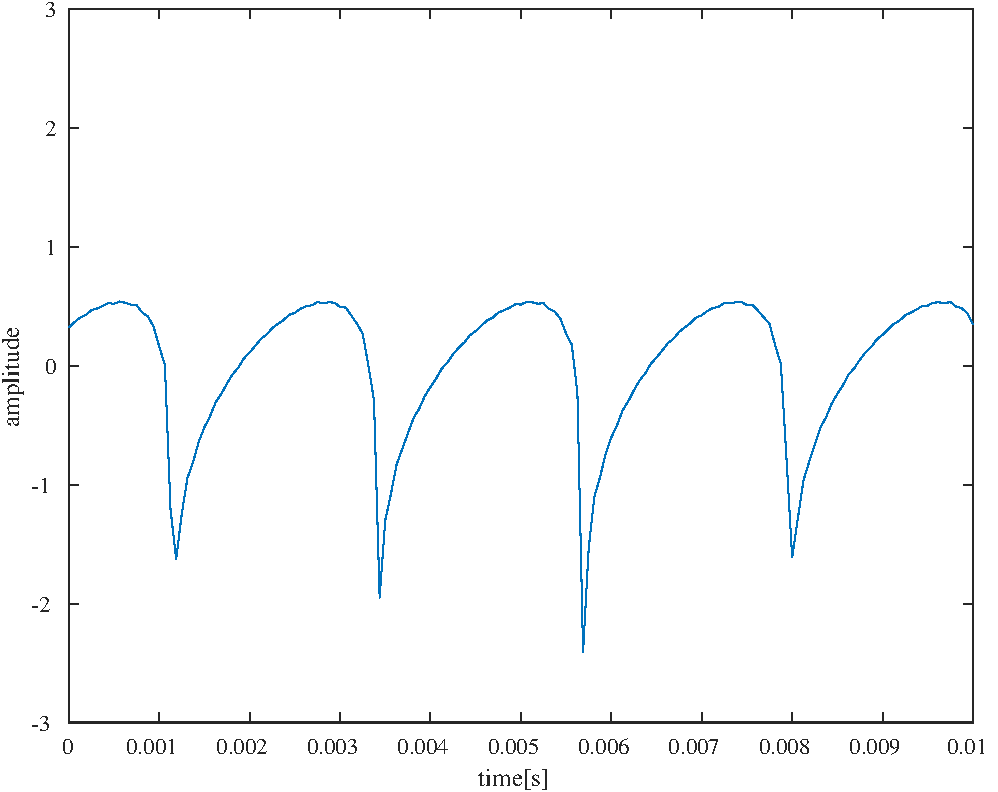
\includegraphics[keepaspectratio,width=\textwidth]{../../Figures/03_22.pdf}
        \subcaption{初期位相\ \(+\pi/4\)}
        \label{fig:実験結果ノコギリ波_p4PI}
    \end{minipage}
    \begin{minipage}{.24\textwidth}
        \centering
        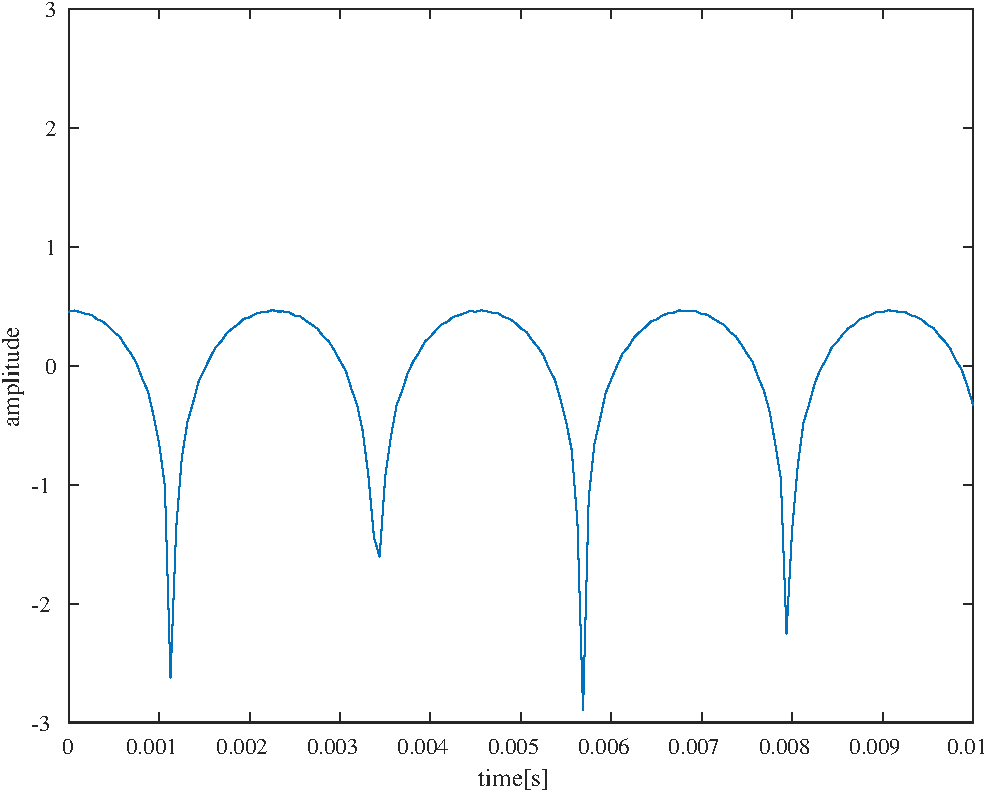
\includegraphics[keepaspectratio,width=\textwidth]{../../Figures/03_23.pdf}
        \subcaption{初期位相\ \(+\pi/2\)}
        \label{fig:実験結果ノコギリ波_p2PI}
    \end{minipage}
    \begin{minipage}{.24\textwidth}
        \centering
        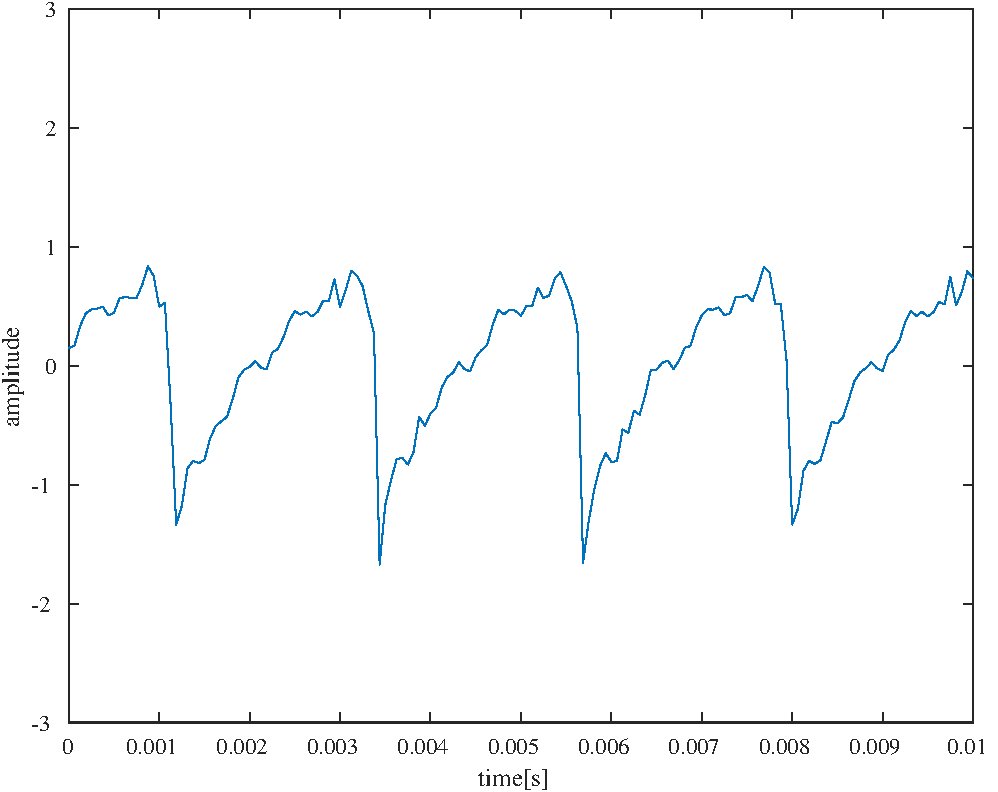
\includegraphics[keepaspectratio,width=\textwidth]{../../Figures/03_24.pdf}
        \subcaption{初期位相\ \texttt{rand}}
        \label{fig:実験結果ノコギリ波_rand}
    \end{minipage}
    \caption{ノコギリ波の初期位相}
    \label{fig:ノコギリ波の初期位相}
\end{figure}
\consideration
純音(正弦波)では初期位相を与えると,その波形は横軸に並行移動する.
しかし,矩形波やノコギリ波は並行移動せずに波形が変わる.これは,矩形波やノコギリ波がさまざまな周波数の高調波から成り立っているからであろう.
また,初期位相を与えた波の振幅が,源波形振幅の2から3倍である理由として,源波形の音波で弱めあっていた点の高調波が並行移動することによって,強めあいに転じたことが考えられる.\par
音量について,振幅と音量は比例する.初期位相を与えた場合,波形の振幅が大きくなるにもかかわらず,音量は小さくなることが分かった.この理由は今後の課題として調査したい.\par
また,実験結果からわかるように,矩形波やノコギリ波に初期位相を与えると,波形が滑らかになるとともに音も滑らかに知覚された.
\section{\kadaicb}\label{sec:\kadaicb}
\purpose
最近のイヤホンやヘッドホンには「ノイズキャンセリング」という機能が搭載されている.これは周りの雑音を音声加工によって軽減する技術である.
この技術は雑音と,それをもとに生成した音の加算合成波を\(0\)にすることで再現している.今回の実験では\matlab を用いて,ある音波に対して合成波が\(0\)になるような音波を生成する.
生成した波と,元となった波の音と波形の違いを明確にする.
\method
\begin{wrapfigure}{r}[0mm]{.3\textwidth}
    \vspace{-2.4cm}
    \centering
    \begin{lstlisting}[caption={モノラルへの変換},label={src:モノラルへの変換},numbers={none}]
% y : N行2列
% ステレオオーディオデータ
mono = y(:,1); % 2列目を削除
    \end{lstlisting}
    \vspace{-.6cm}
\end{wrapfigure}
正弦波\(y_1=\sin(x)\)に対して,合成波が\(0\)になるような正弦波は,\(y_2=-\sin(x)\)であり,\(y_1\)と\(-1\)の積である.無論,\(y_1+y_2=0\)となる.\par
これは正弦波に限った話ではない.任意の実数値関数\(f:x\longrightarrow f(x)\quad(x\in\mathbb{R})\)に対して,横軸\(x\),縦軸\(f(x)\)のグラフを描画する.
横軸を対称の軸として,値\(f(x)\)を線対称移動すると\(-f(x)\)になる.つまり,ある音波に対して,その波の値と\(-1\)の積を取った値を加算合成すれば,合成波は\(0\)になる.
\paragraph{実装}
音波Aの各要素と\(-1\)の積を演算するには,\texttt{A\underline{.*}(-1)}と入力する.\ \underline{\texttt{.*}}\ は各要素との積をとる演算子である.
また,録音した音声がステレオオーディオの場合,モノラルオーディオに変換する(\srcref{src:モノラルへの変換}).
\paragraph{実験の内容}
今回は母音「\texttt{a}」,「\texttt{i}」の2つを処理する.それぞれ振幅データと\(-1\)の積をとる.処理後の波形,元の波形,合成波の,それぞれ一部描画する.
「\texttt{a}」の音声データを\texttt{sound1.wav},「\texttt{i}」の音声データを\texttt{sound2.wav}に格納している.\scall\sref{src:03_02_a},\sref{src:03_02_i}.
\result
波形を\figref{fig:処理前後の波形_a},\figref{fig:処理前後の波形_i}に示す.聴音確認の結果,処理の前後で音の変化は確認できなかった.
さらに,合成波(\texttt{synthetic wave})は常に\(0\)であった.
\begin{figure}[h]
    \centering
    \begin{minipage}[b]{.48\textwidth}
        \centering
        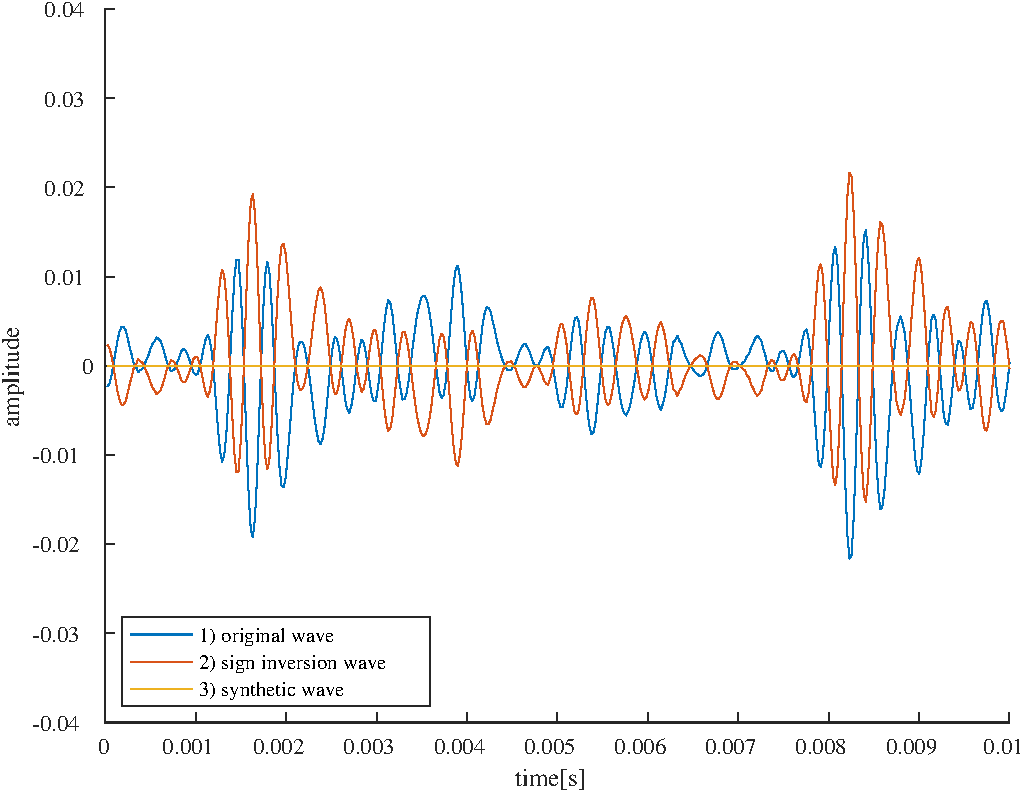
\includegraphics[keepaspectratio,width=\textwidth]{../../Figures/03_2_a.pdf}
        \caption{処理前後の波形:「\texttt{a}」}
        \label{fig:処理前後の波形_a}
    \end{minipage}
    \begin{minipage}[b]{.48\textwidth}
        \centering
        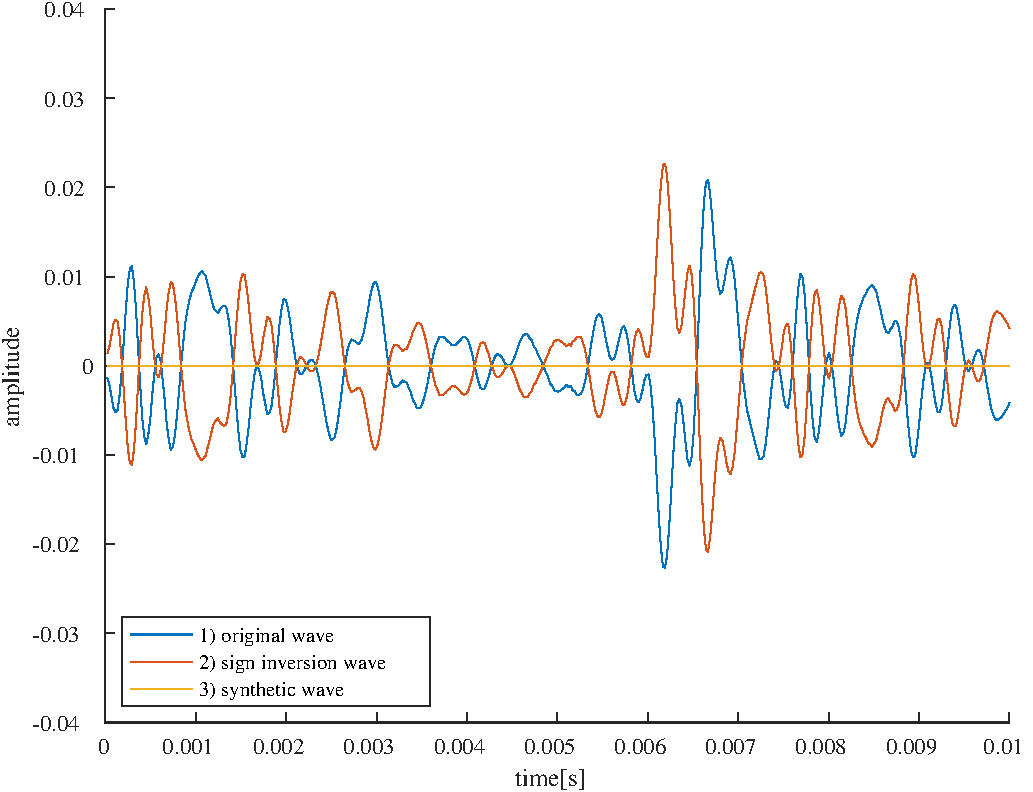
\includegraphics[keepaspectratio,width=\textwidth]{../../Figures/03_2_i.pdf}
        \caption{処理前後の波形「\texttt{i}」}
        \label{fig:処理前後の波形_i}
    \end{minipage}
\end{figure}
\consideration
結果より,合成波が\(0\)であることを確認した.上下(正負)を逆にして生成した音波と元となった音波を合成すると無音になる.
波の正負が反転しても,聞こえ方は変わらないと知覚する理由として,ヒトの聴覚は振動を「音圧」としてとらえていることが考えられる.
\section{\kadaicc}\label{sec:\kadaicc}
\purpose

\begin{wrapfigure}{r}[0mm]{.3\textwidth}
    \vspace{-2cm}
    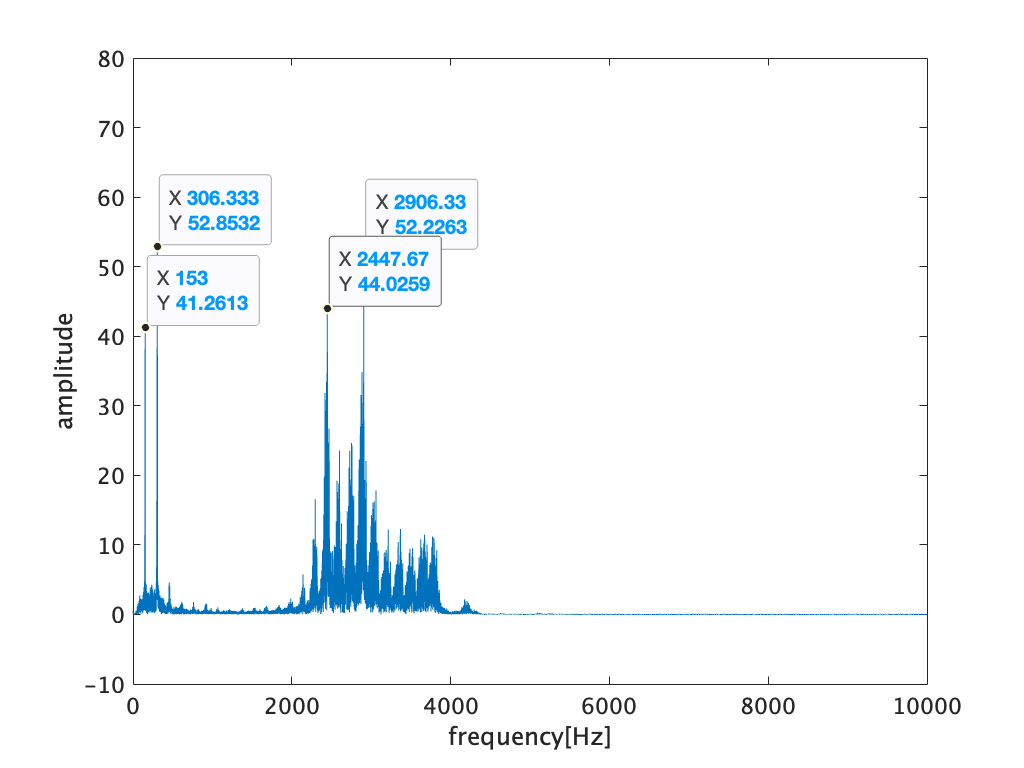
\includegraphics[keepaspectratio,width=.3\textwidth]{../../Figures/03_00_ex.png}
    \caption{縦横軸の値を抽出する}
    \label{fig:縦横軸の値を抽出する}
    \vspace{-2cm}
\end{wrapfigure}

\ref{sec:\kadaiad}章より,任意の波はフーリエ変換し,周波数解析できる.
今回の実験では,音声を周波数解析し,振幅スペクトル上でピークのある周波数および振幅データを抽出した後,それらを元に音波を生成する.生成した音波と元となった音波の違いを聴き比べる.
\method
\ref{sec:\kadaicb}章で用いた\texttt{sound1.wav},\texttt{sound2.wav}に対して,周波数解析する.
\matlab の\texttt{plot}関数で出力したグラフは,ピークの点をクリックするとその点の値を取り出すことができる(\figref{fig:縦横軸の値を抽出する}).今回は,\(0\textrm{Hz}\)から\(10000\textrm{Hz}\)までを振幅スペクトルとして書き出す.
取り出した点を行列に保存し,その振幅と周波数から純音を生成する.
このとき,時刻\(t\)に対して,周波数\(f\)と振幅\(A\)に対して,\(f(t) = A\sin(2\pi ft)\)と表せること,すべての波は正弦波の和で表せることをもとに,生成した純音を合成し,音波を作成する.\scall\sref{src:03_03}.
\result
聴音確認の結果,合成後の音は,「\texttt{a}」,「\texttt{i}」と聞こえたが,原音波に比べて「ガサガサ」とした音であった.
\begin{figure}[H]
    \centering
    \begin{minipage}{.3\textwidth}
        \centering
        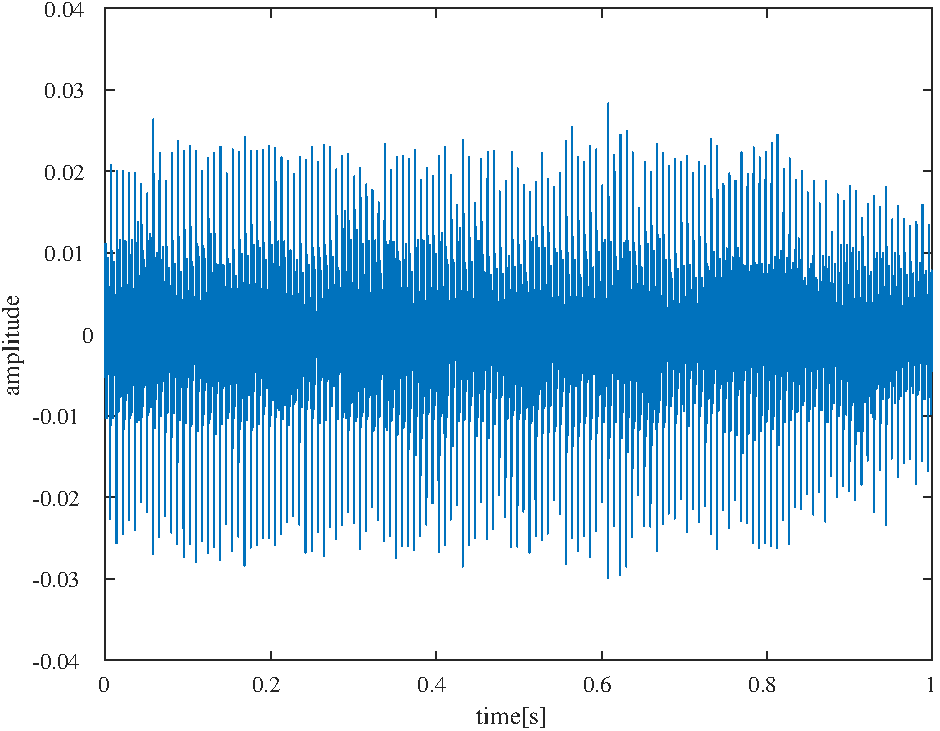
\includegraphics[keepaspectratio,width=\textwidth]{../../Figures/03_30_0a.pdf}
        \subcaption{源音波(一部)}
    \end{minipage}
    \begin{minipage}{.3\textwidth}
        \centering
        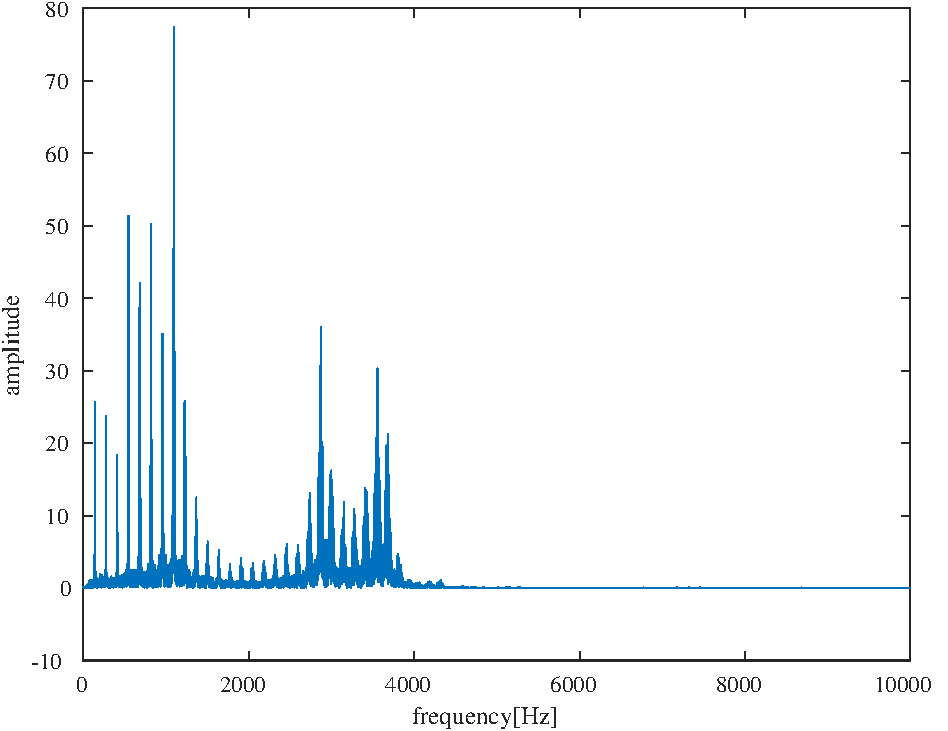
\includegraphics[keepaspectratio,width=\textwidth]{../../Figures/03_30_afft.pdf}
        \subcaption{振幅スペクトルの絶対値}
        \label{fig:振幅スペクトルの絶対値_a}
    \end{minipage}
    \begin{minipage}{.3\textwidth}
        \centering
        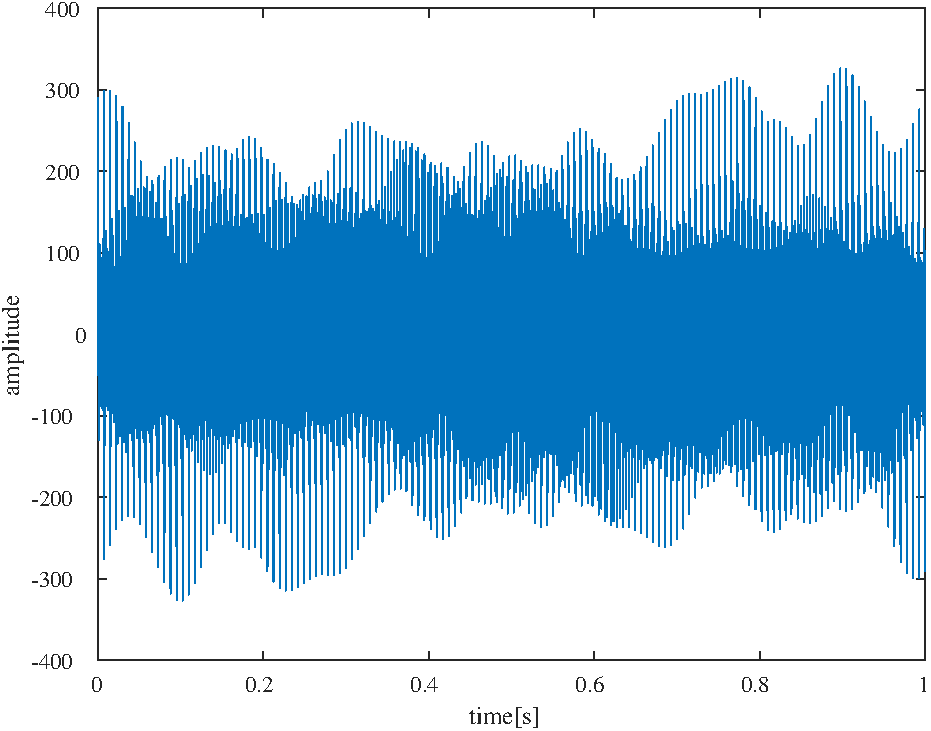
\includegraphics[keepaspectratio,width=\textwidth]{../../Figures/03_32_a.pdf}
        \subcaption{合成音波(一部)}
    \end{minipage}
    \caption{母音「\texttt{a}」}
    \label{fig:合成音声_a}
    \begin{minipage}{.3\textwidth}
        \centering
        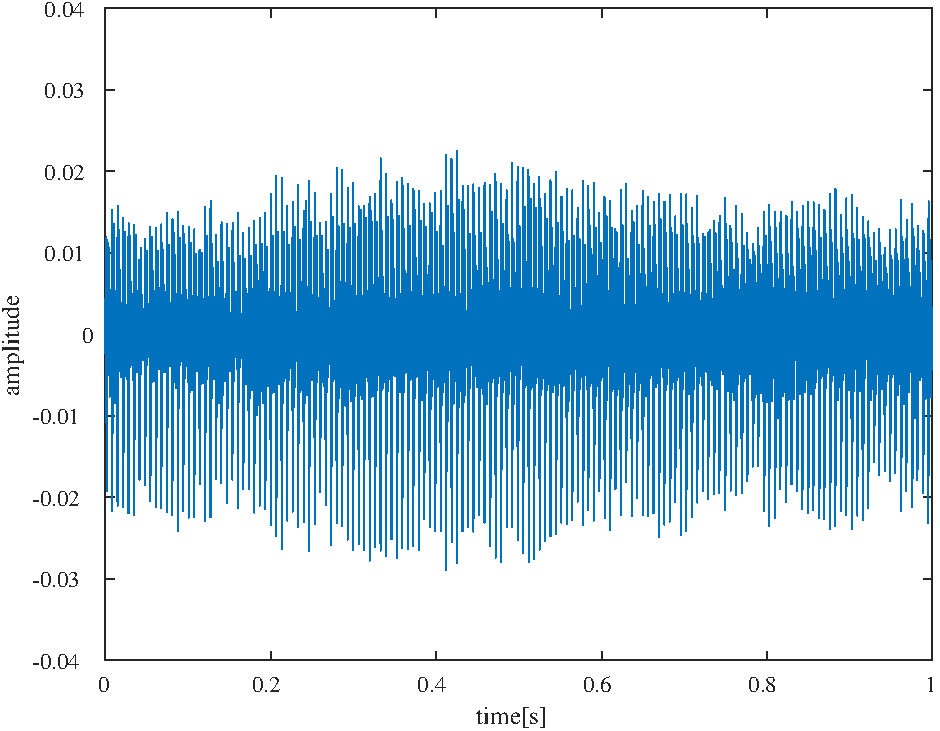
\includegraphics[keepaspectratio,width=\textwidth]{../../Figures/03_30_0i.pdf}
        \subcaption{源音波(一部)}
    \end{minipage}
    \begin{minipage}{.3\textwidth}
        \centering
        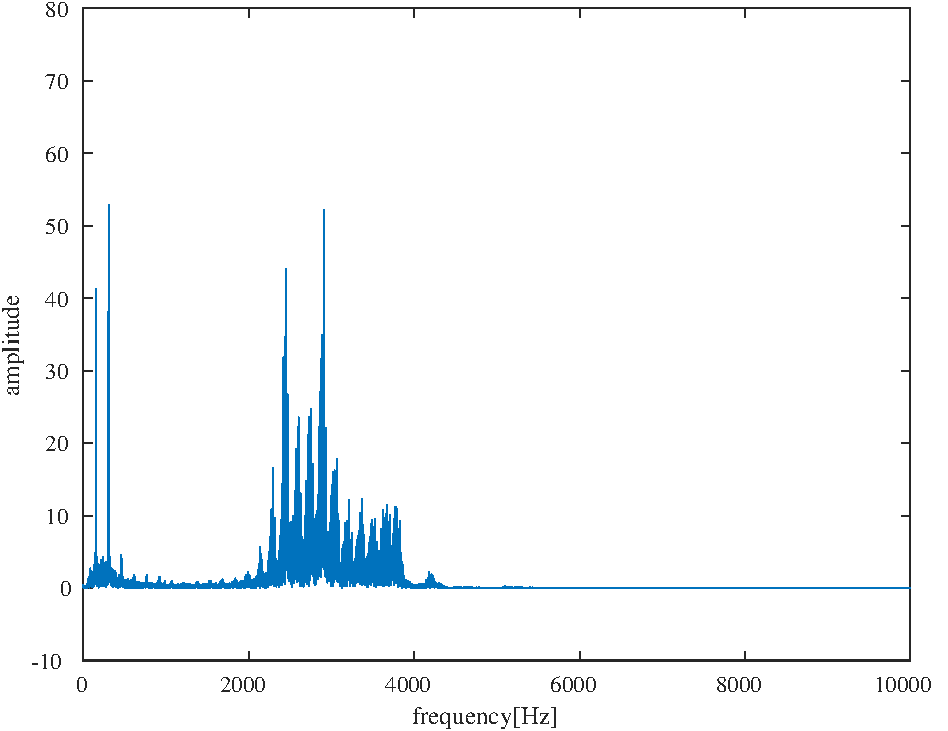
\includegraphics[keepaspectratio,width=\textwidth]{../../Figures/03_31_ifft.pdf}
        \subcaption{振幅スペクトルの絶対値}
        \label{fig:振幅スペクトルの絶対値_i}
    \end{minipage}
    \begin{minipage}{.3\textwidth}
        \centering
        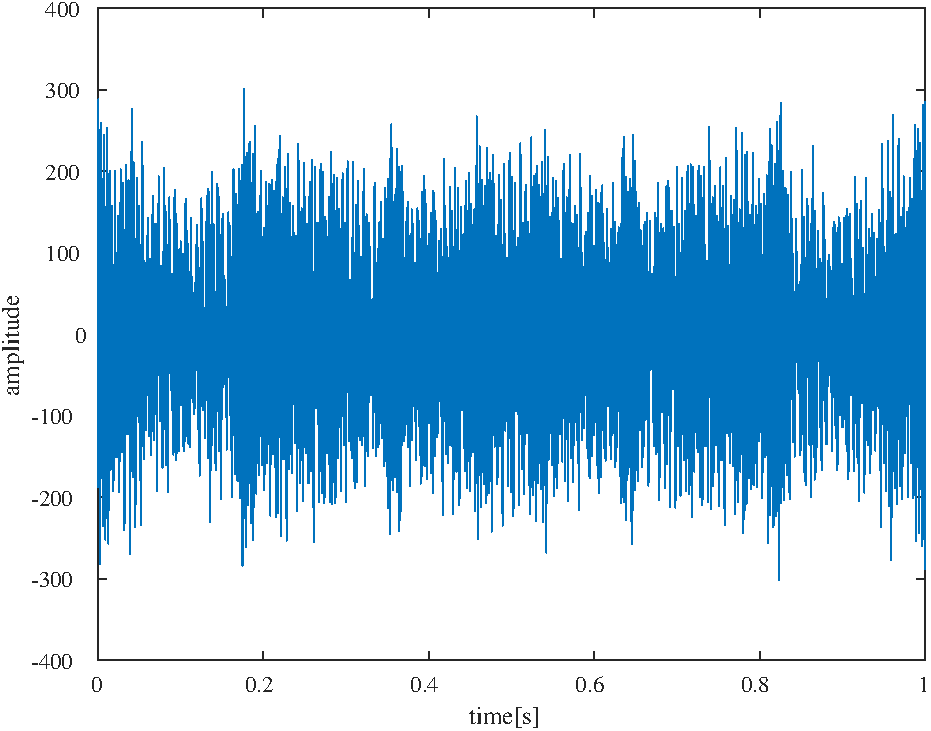
\includegraphics[keepaspectratio,width=\textwidth]{../../Figures/03_33_i.pdf}
        \subcaption{合成音波(一部)}
    \end{minipage}
    \caption{母音「\texttt{i}」}
    \label{fig:合成音声_i}
\end{figure}
\consideration
源音波と合成音波を比べてみると,縦軸が異なる.これは,特定の周波数を取り出すことによって,弱めあう正弦波を合成しなかったためであろう.
また,「ガサガサ」と音が聞こえるのは,抽出していない大部分の高調波成分が欠け,「本来必要な周波数の正弦波がないこと」が原因であろう.
